\section{ $\Mtilde$ and Mass Window Selection}
\label{sec:masswindow}

In order to increase the sensitivity of the resonant analysis, we perform a cut on the 4-body invariant mass before the signal extraction with the 2D fit.
In the Run I analysis, the 4-body invariant mass was corrected with a kinematic fit, to mitigate the effects of the low mass resolution of the dijet system.
However, it has been seen that this method is too reliant on the a-priori set of energy and spatial resolutions for the jets in that analysis (these resolutions must be measured in situ, since they are kinematic dependent).
One solution for this was to use instead the variable $\Mtilde$, defined as:

\begin{equation}
\Mtilde = \Mjjgg - \Mjj - \Mgg + 250 \text{ GeV}.
\end{equation}

This variable performs a kinematic fit "by hand", by effectively scaling the dijet and diphoton invariant masses to 125 GeV. 
In order to quantify the improvementof this variable with respect to other 4-body invariant mass reconstructions, we calculate the width of the smallest interval that covers $68\%$ of the signal shape in each reconstruction method. 
We compare $\Mtilde$ with the standard $\Mjjgg$ and with $\Mjjgg_{KF}$, which is reconstructed with a kinematic fit in $\Mjj$, which tries to vary the jets within their uncertainties to achieve $\Mjj = 125$ GeV. 
The widths are compared in Figure \ref{fig:mxwidth}. 

\begin{figure*}[h]
  \centering
  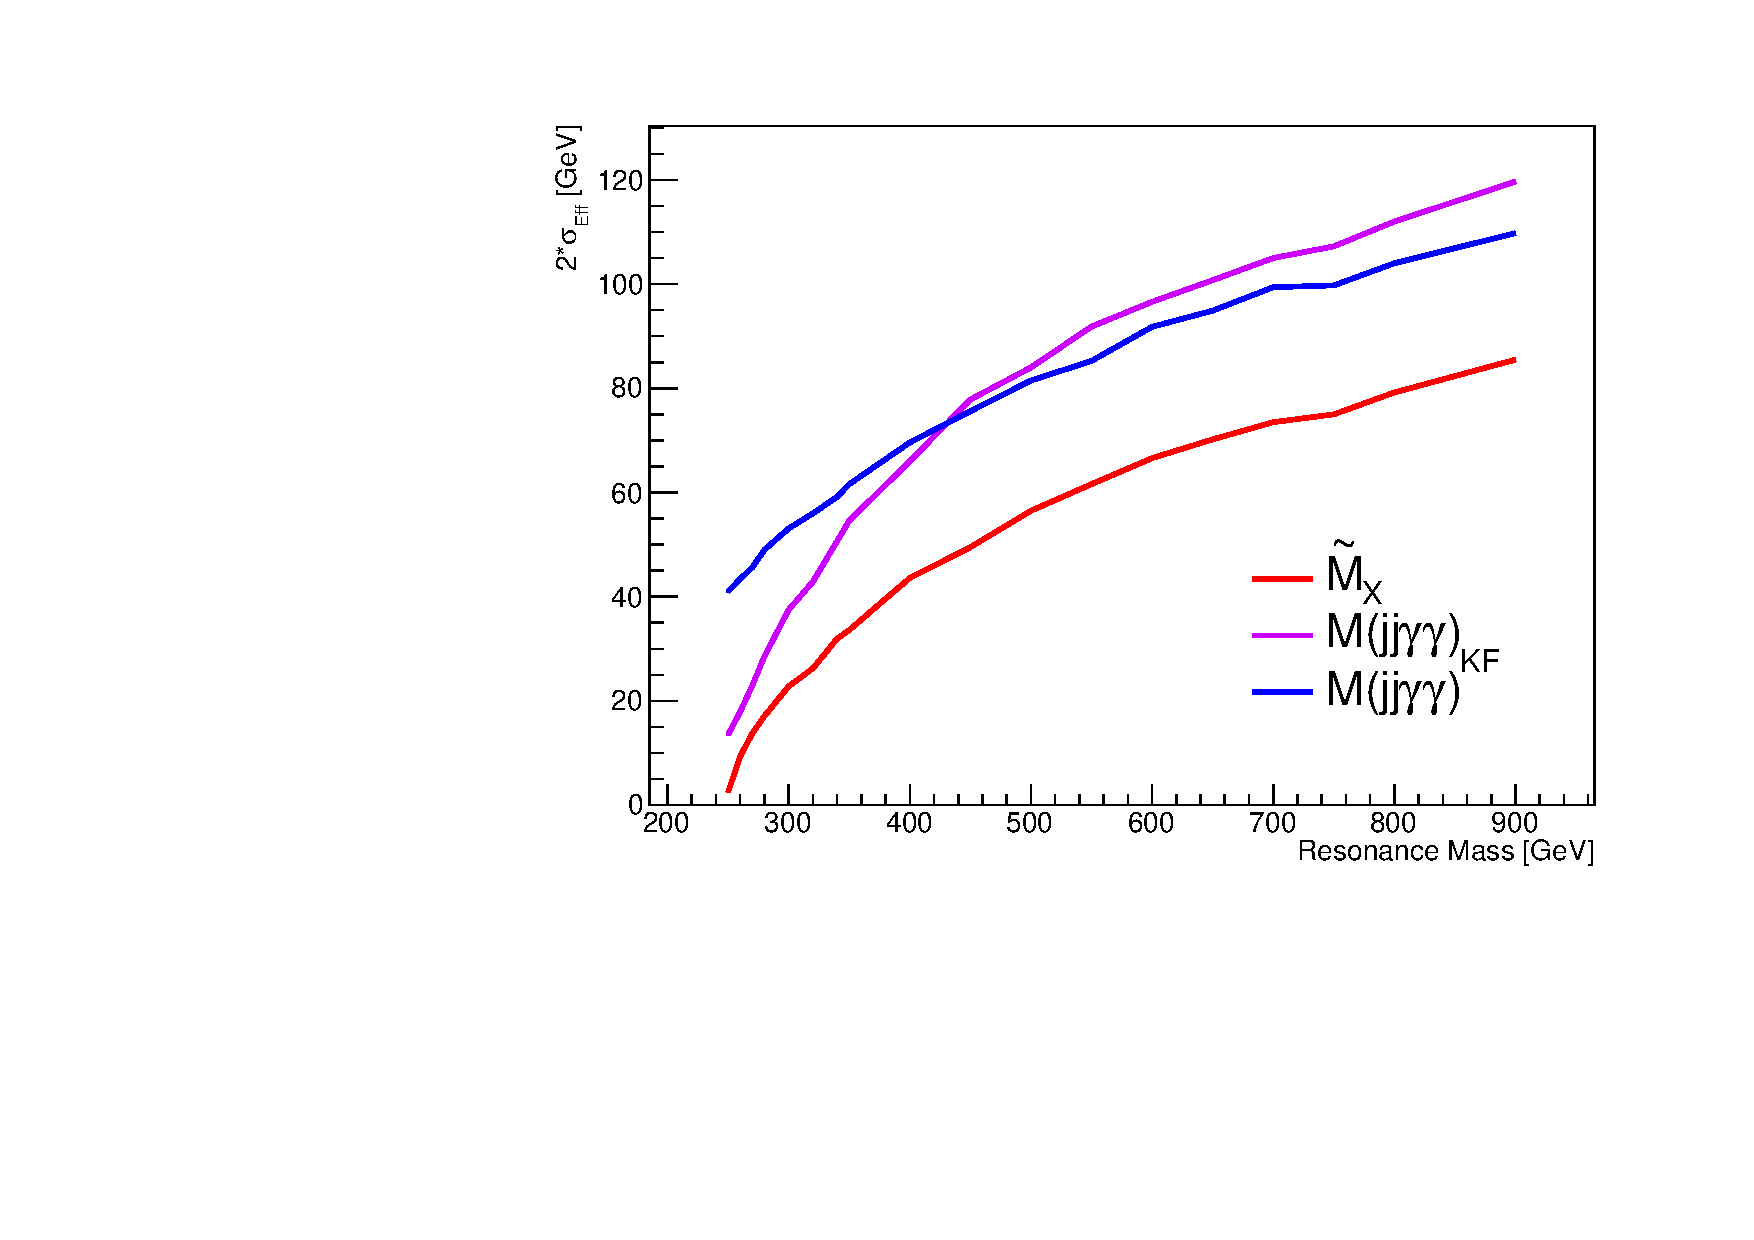
\includegraphics[width=0.6\textwidth]{figures/sec-window/width_67_prime.pdf}\hfil
  \caption{Different 4-body mass widths: $\Mtilde$, $\Mjjgg$ with kinematic fit, and $\Mjjgg$ with no extra corrections.}
  \label{fig:mxwidth}
\end{figure*}

The effect of reconstructing the 4-body invariant mass with $\Mtilde$ on the signal shape can be seen in \ref{fig:mx}. 
The figure shows that the $\Mtilde$ reconstruction yields a better performing resolution for the 4-body invariant mass reconstruction, meaning that we can perform tighter cuts on it and increase the signal/background for each signal mass point.

One extra check we must do while using this variable is to make sure there are no unexpected effects on the background shapes. 
The effect of $\Mtilde$ is similar to the kinematic fitted $\Mjjgg$, but more pronounced, which is the sharp kinematic cut around the $\Mtilde = 250$ GeV point. This can be seen in the figures in section \ref{sec:control}..

\begin{figure*}[h]
  \centering
  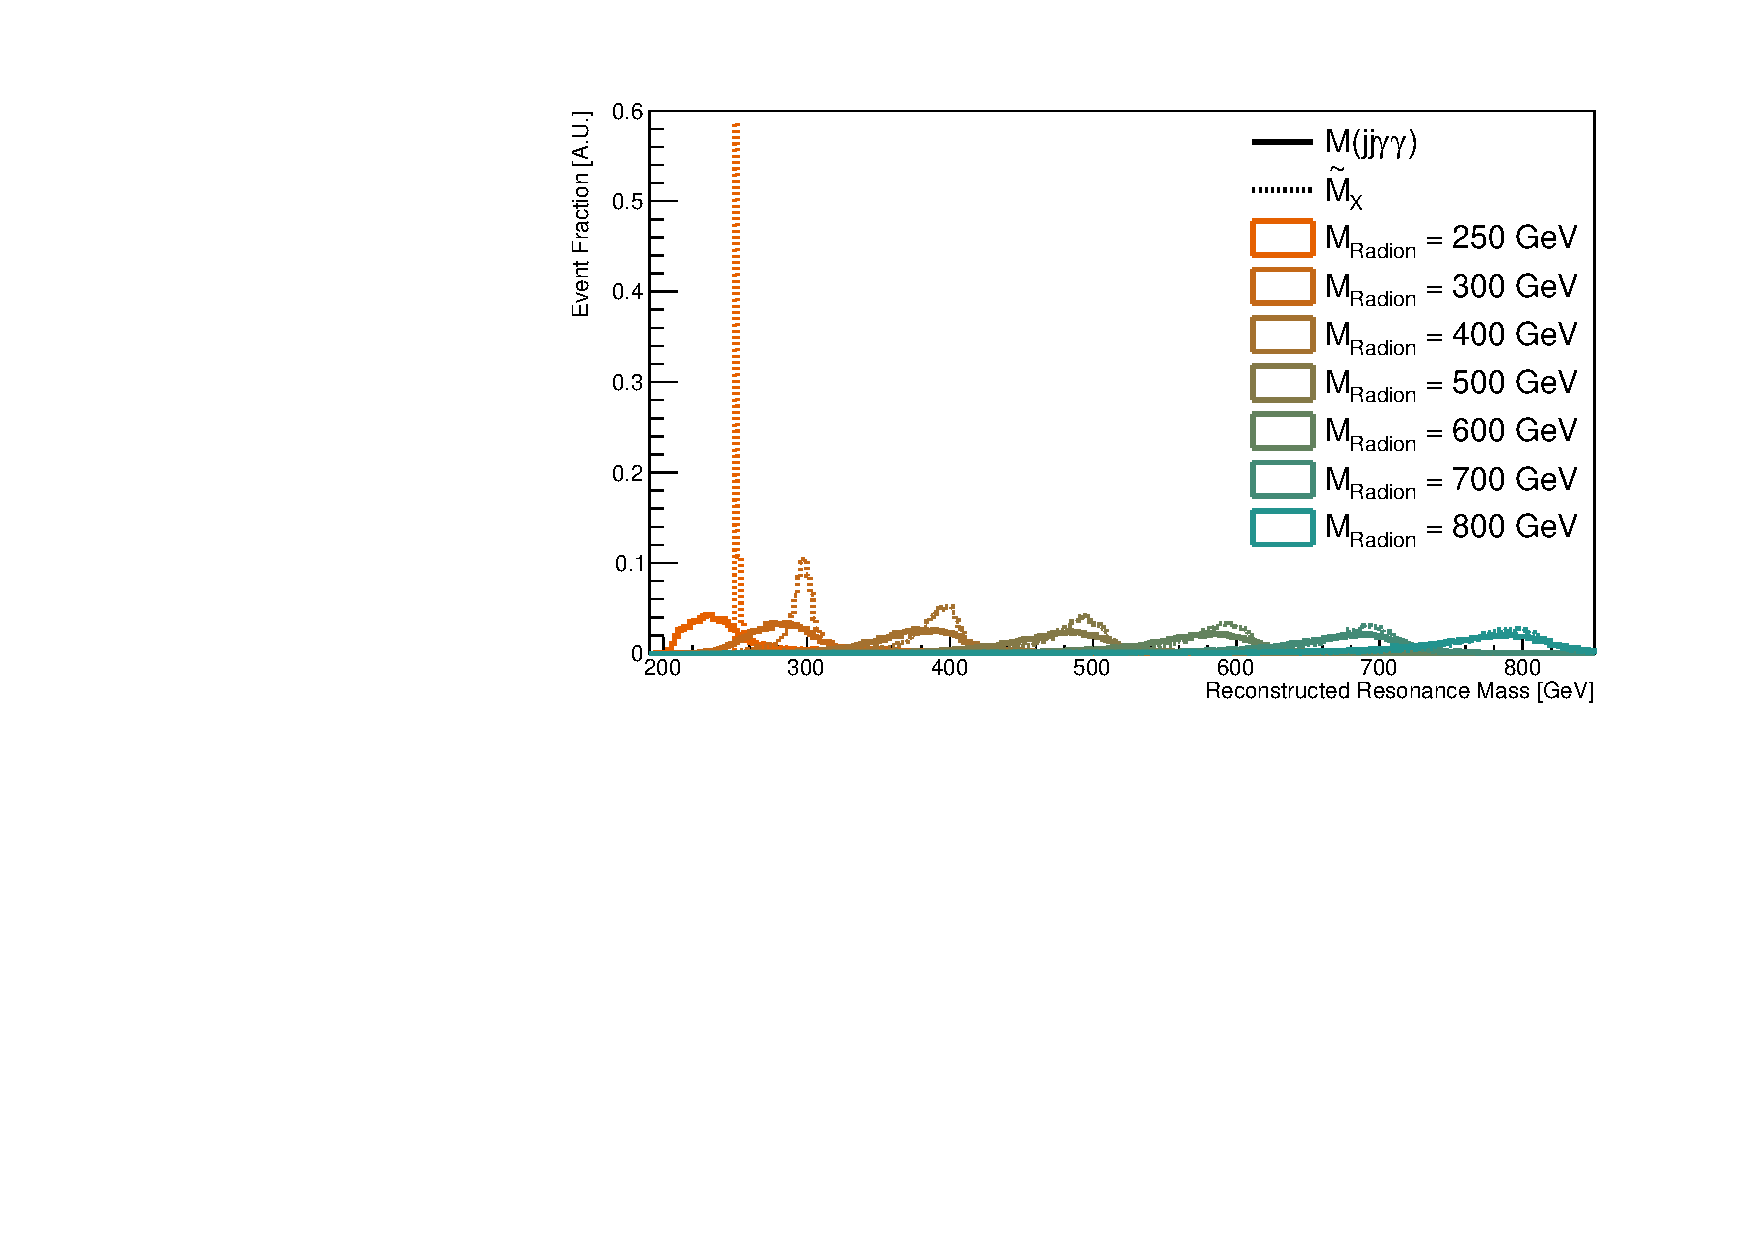
\includegraphics[width=0.6\textwidth]{figures/sec-window/prplot.pdf}\hfil
  \caption{Different 4-body mass reconstructions: $\Mtilde$ (dotted line), $\Mjjgg$ with kinematic fit (dashed line), and $\Mjjgg$ with no extra correction (full line). Signals for different radion masses are shown. The normalizations are such that the non-corrected mass peaks at 1 (same normalization for different reconstructions in each mass point). This plot is made after full selection, in the b-tagging signal region (at least one medium b-tagged jet).}
  \label{fig:mx}
\end{figure*}

It has also been observed that, for the non-resonant signal samples, the $\Mtilde$ variable approaches the generator level HH invariant mass distribution more so than the kinematic fitted $\Mjjgg$ and the default 4-body invariant mass. This can be seen in figure \ref{fig:mxnonres}. For this, $\Mtilde$ will also be used in the non-resonant analysis.

\begin{figure*}[h]
  \centering
  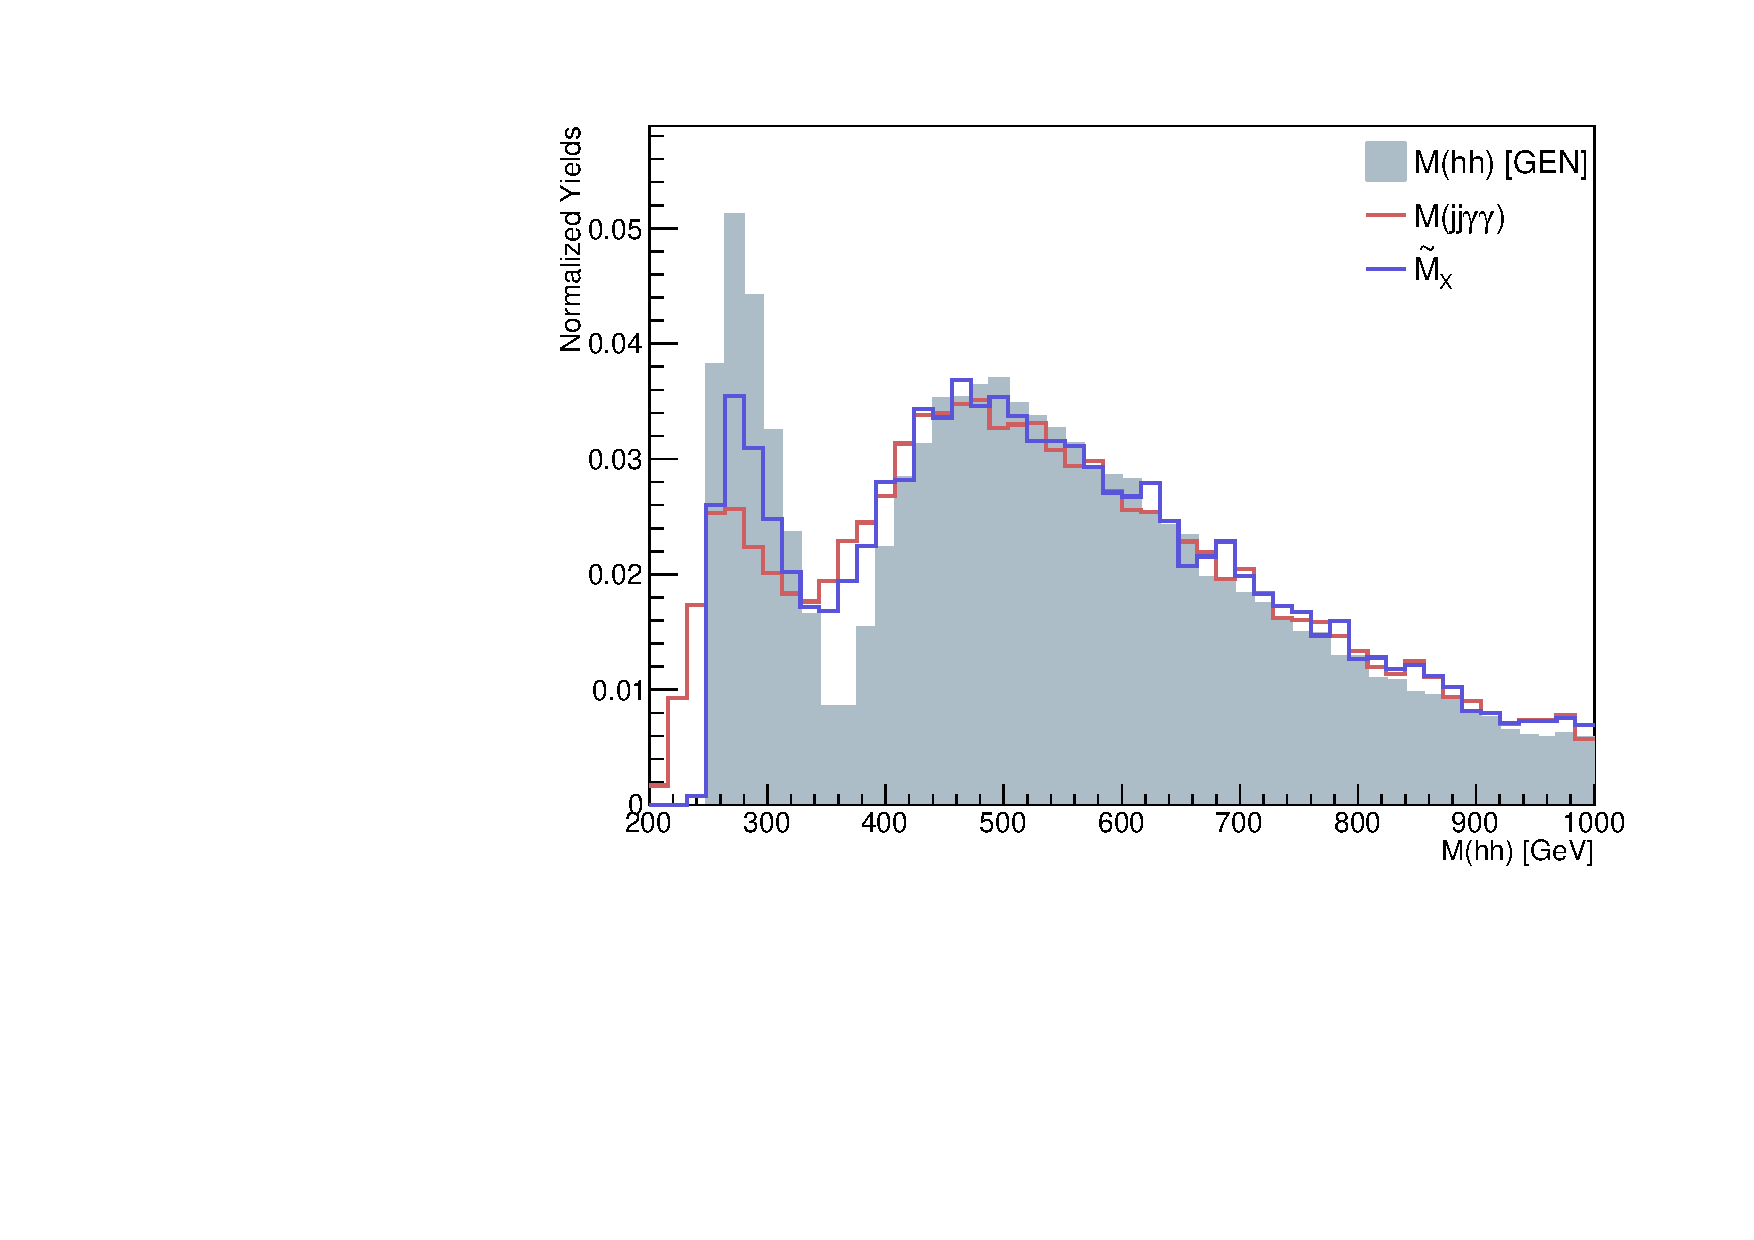
\includegraphics[width=0.45\textwidth]{figures/sec-window/nonresmx.pdf}\hfil
  \caption{Behavior of $\Mtilde$, $\Mggjj$ and GEN-level $M(hh)$. WARNING - THIS IS THE 2015 PLOT}
  \label{fig:mxnonres}
\end{figure*}

One desirable effect of the $\Mtilde$ definition in this version of the analysis, compared to the 2015 definition (which only scaled the $\Mjj$ value as in $\Mtilde = \Mjjgg - \Mjj + 125$ GeV), is that a $\Mtilde$ selection does not bias $\Mgg$ and $\Mjj$. 
This can be seen in the 2D plots of $\Mtilde:\Mgg$ and $\Mtilde:\Mjj$ in Figure \ref{fig:mx2d}. 

\begin{figure*}[h]
  \centering
  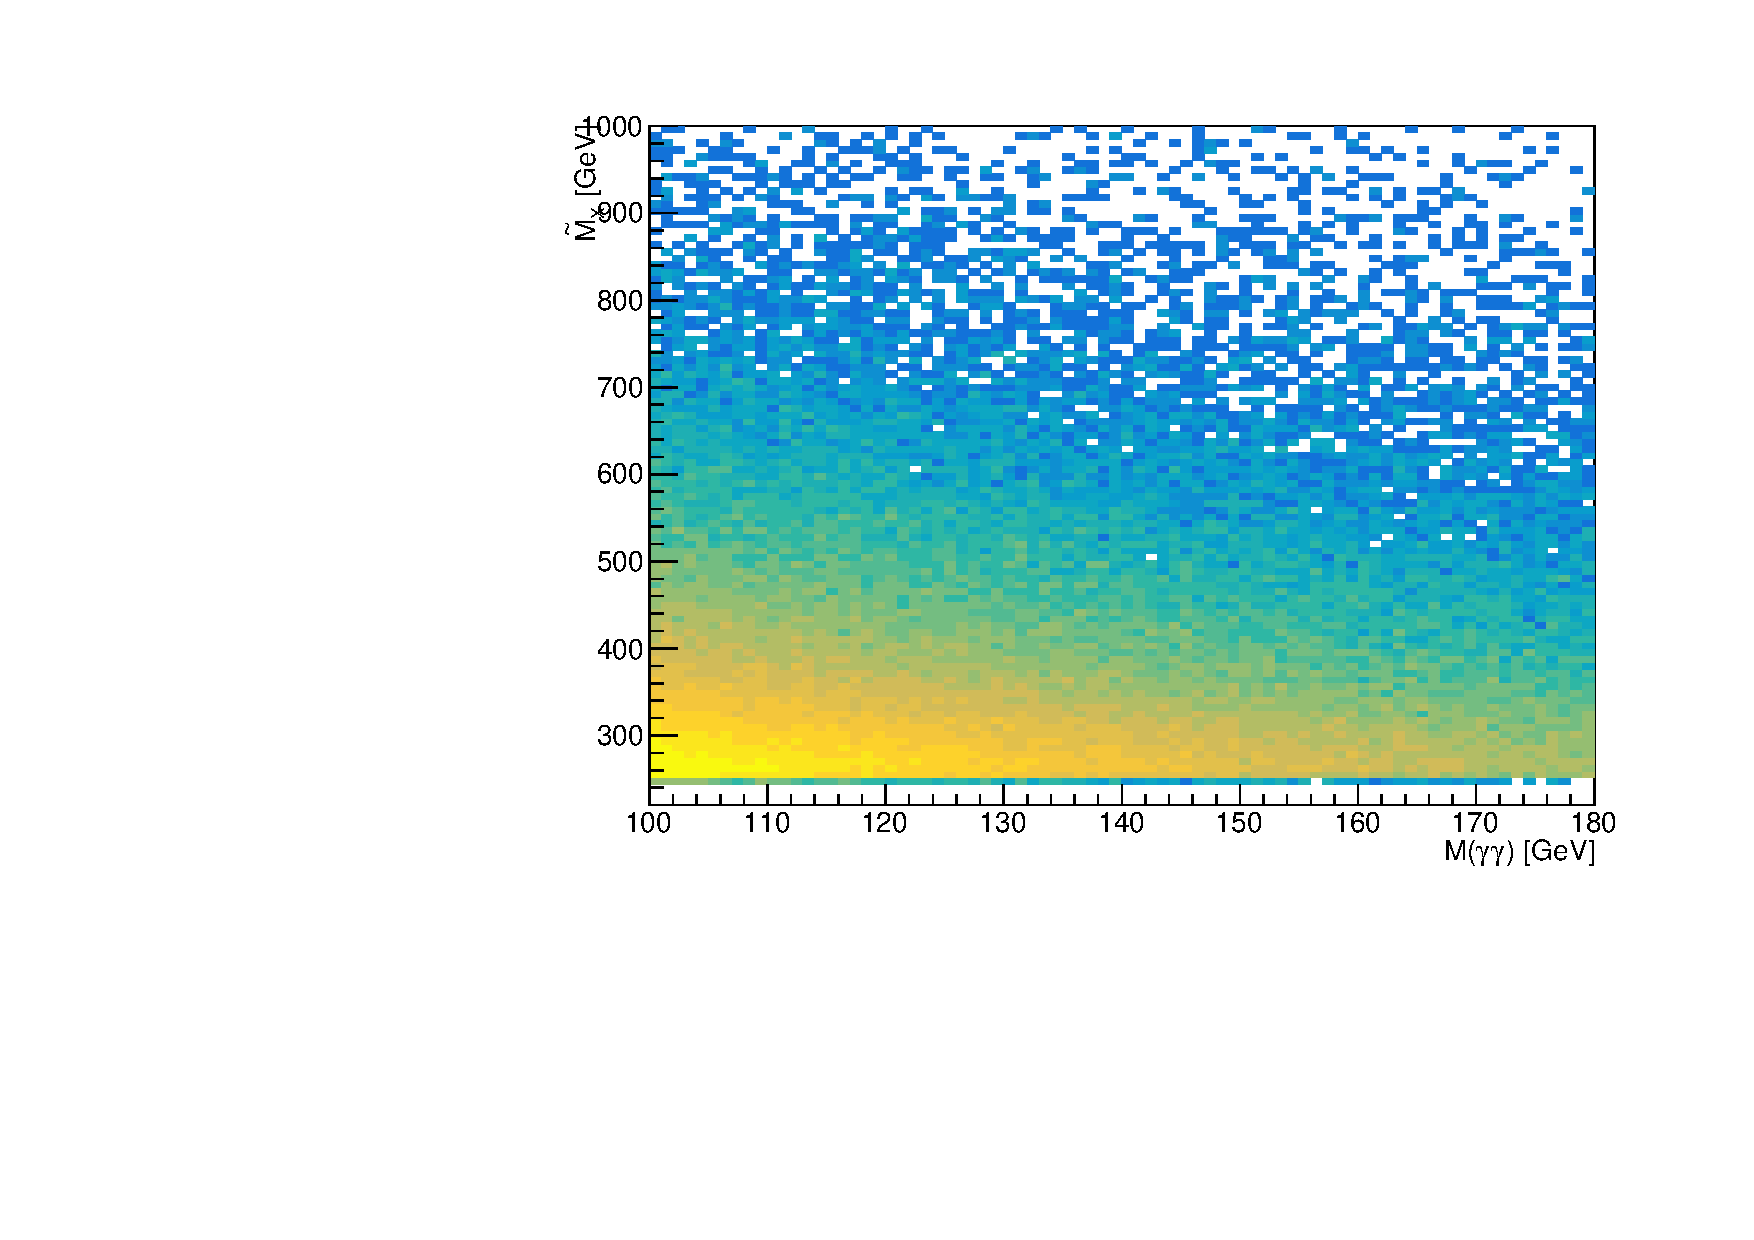
\includegraphics[width=0.45\textwidth]{figures/sec-window/mgg2d.pdf}\hfil
  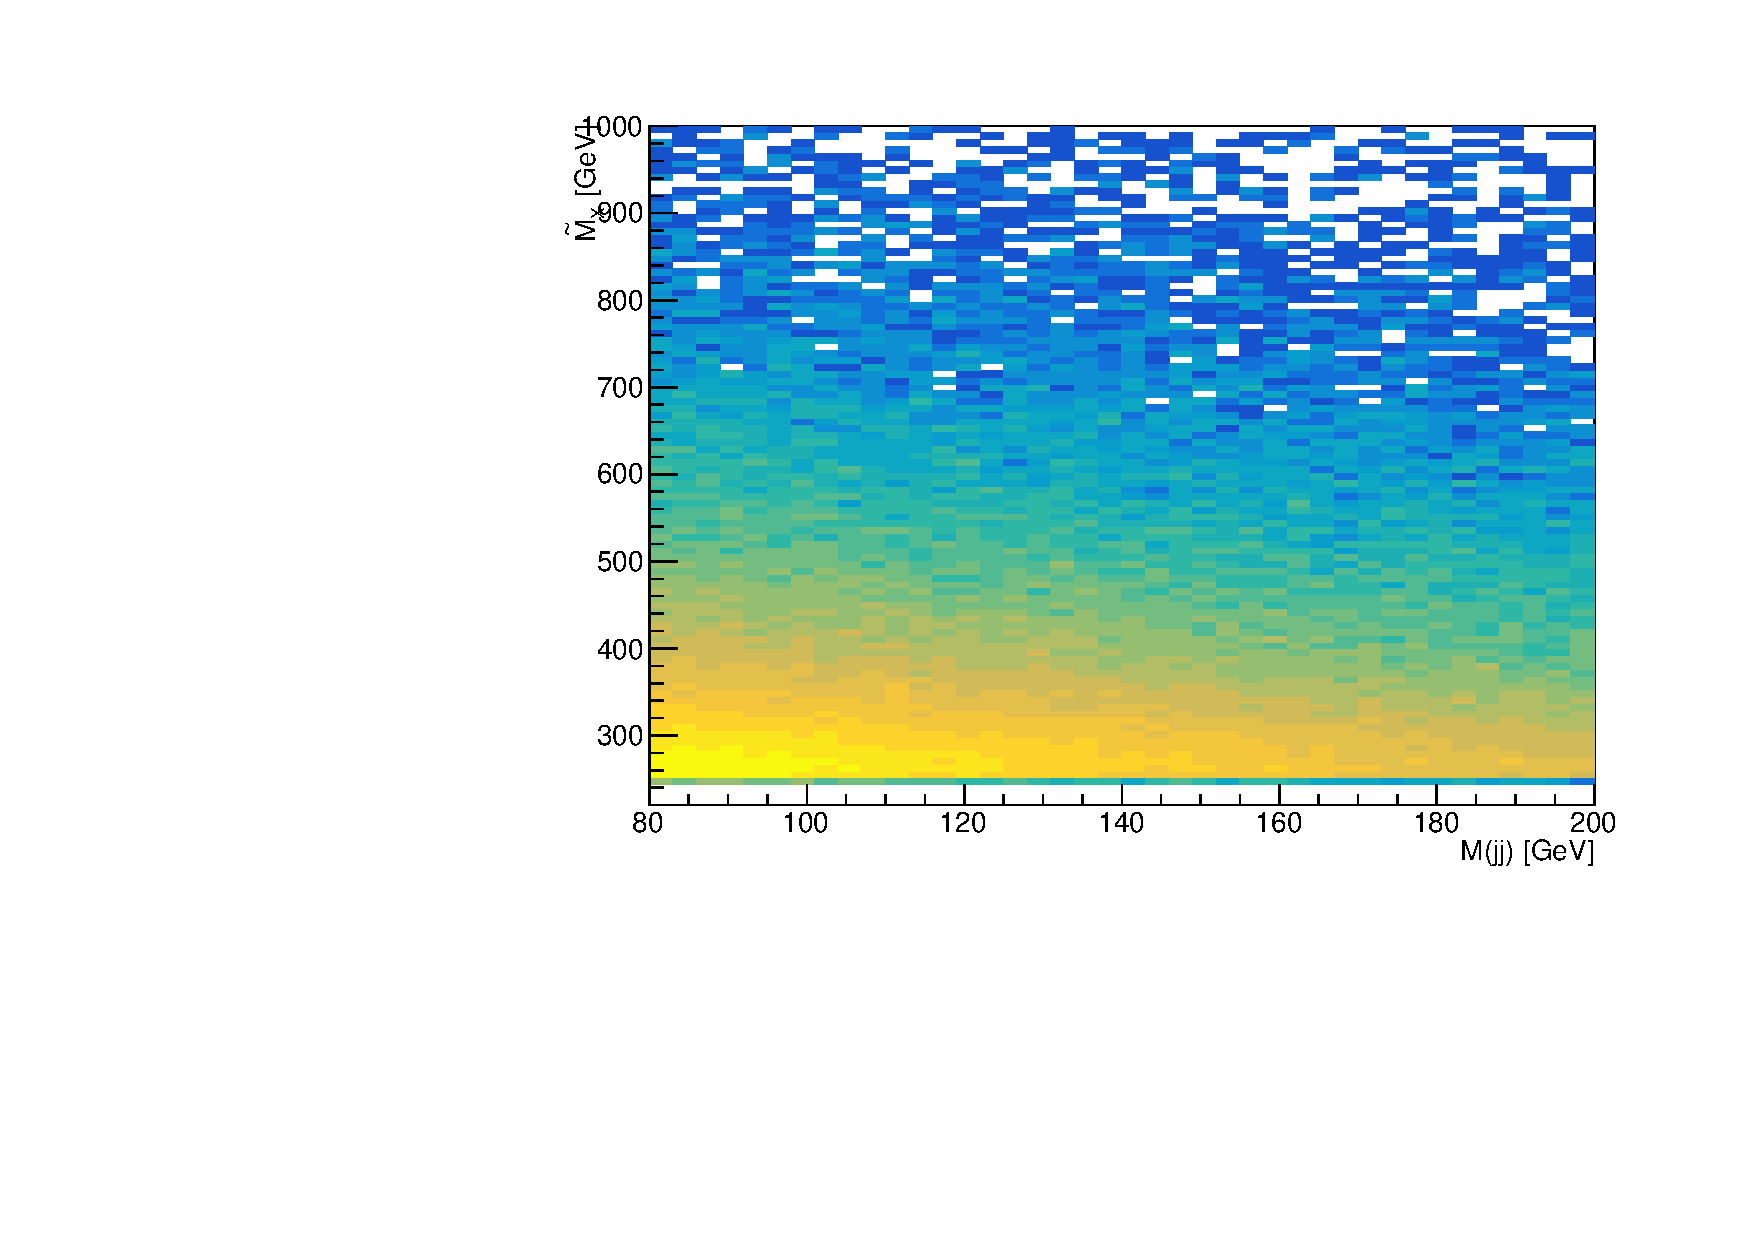
\includegraphics[width=0.45\textwidth]{figures/sec-window/mjj2d.pdf}\hfil
  \caption{$\Mtilde:\Mgg$ and $\Mtilde:\Mjj$ in the photon control region, scaled to unity and Z-axis in log scale. }
  \label{fig:mx2d}
\end{figure*}

With $\Mtilde$, we can improve the resonant analysis by tightening the signal region around the 4-body resonance mass (mass window). 
Through limits optimization, it has been checked that constructing a mass window with the smallest interval that covers $60\%$ of the signal shape provides the best sensitivity. 
The size of these intervals, as a function of the hypothesis mass, is seen in Figure \ref{fig:masswindowwidths}. 

\begin{figure*}[h]
  \centering
  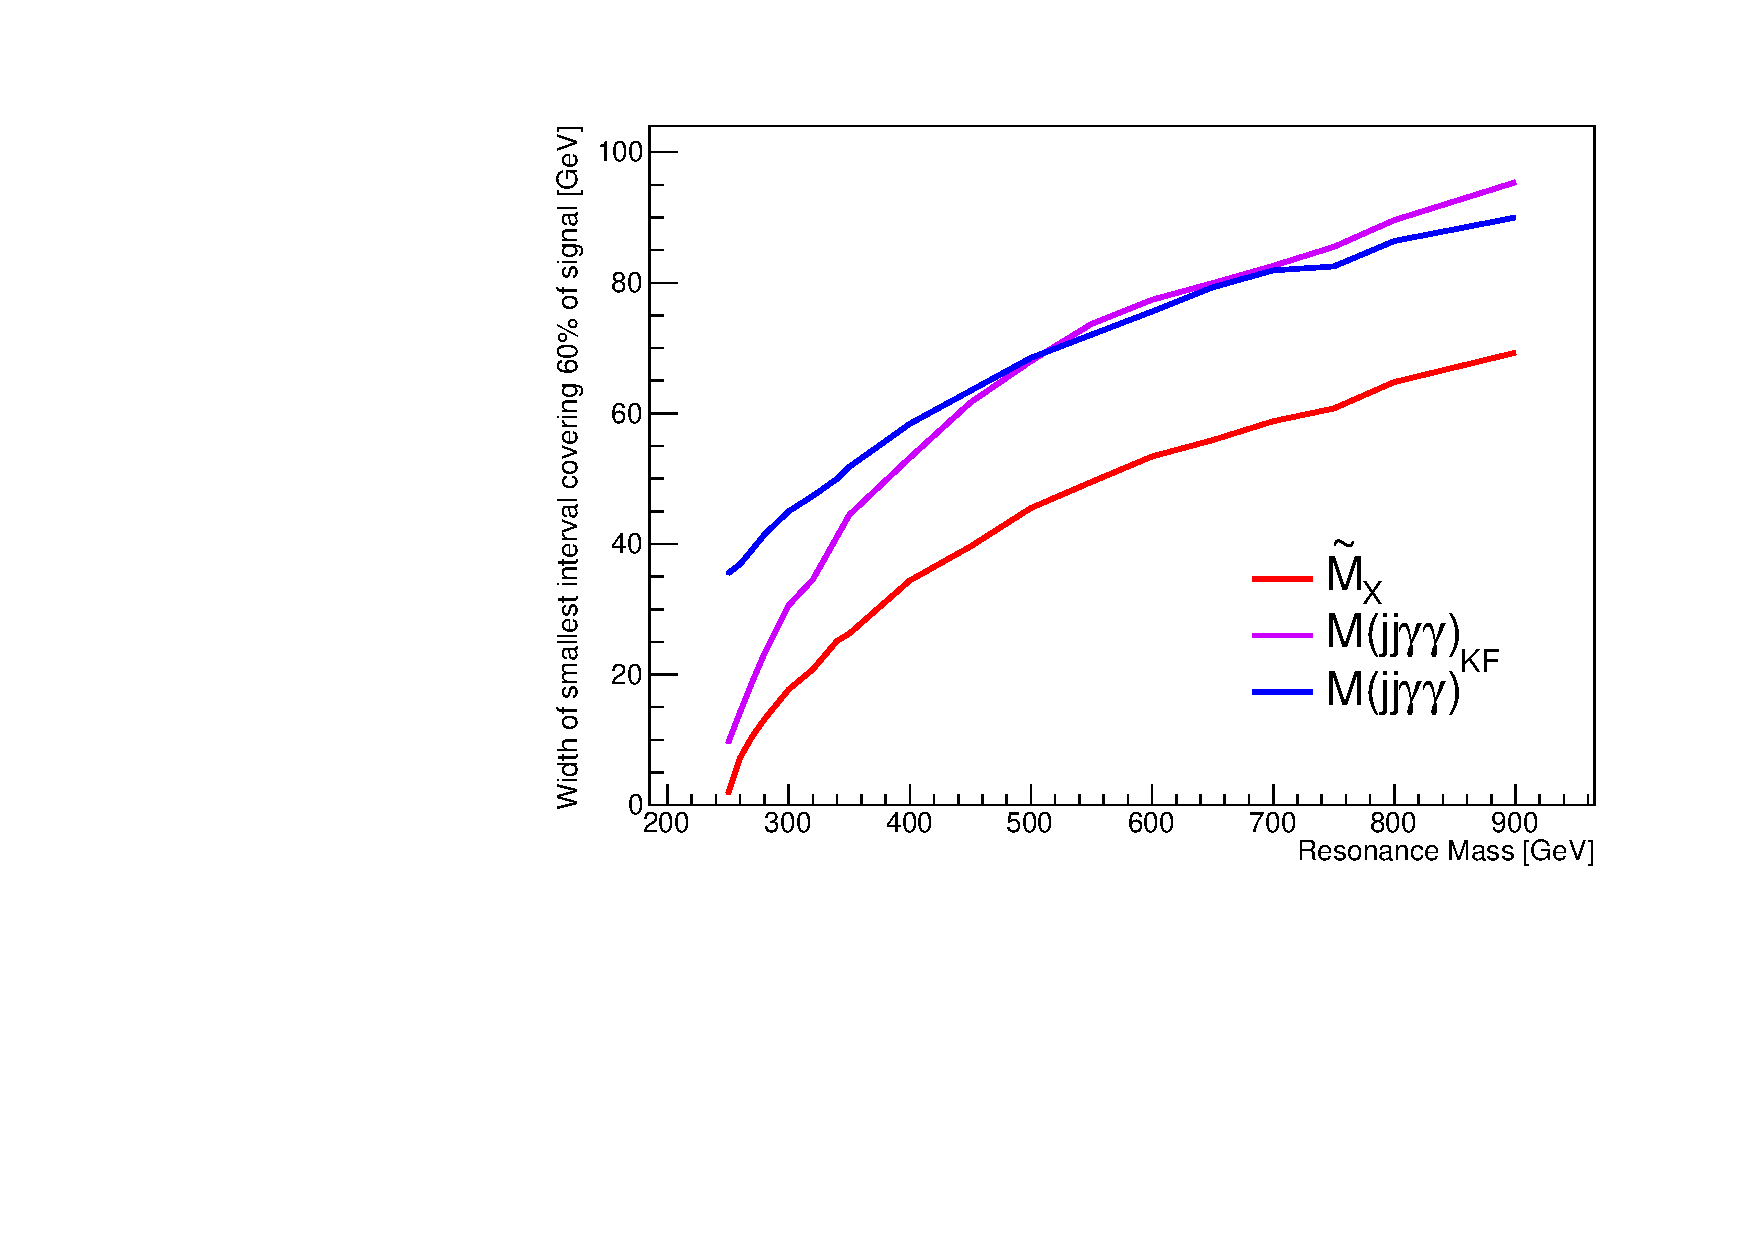
\includegraphics[width=0.45\textwidth]{figures/sec-window/width_60_prime.pdf}\hfil

  \caption{Mass window sizes as a function of the resonance mass. }
  \label{fig:masswindowwidths}
\end{figure*}

We implement this mass window by requiring that $W_{-} < \Mtilde < W_{+}$. 
$W_{\pm}$ are calculated based on the widths defined in Figure \ref{fig:masswindowwidths}. 
We fit $W_{\pm}$ with a 3rd degree polynomial so that the mass windows can be defined functionally based on the mass hypothesis. 
These fits, and, therefore, the definition of $W_{\pm}$ can be seen in Figure \ref{fig:masswindowfit}. 
$W_{\pm}$ can be infered through the Y-axis of \ref{fig:masswindowfit}, $W_{-}$ is defined by the blue curve and $W_{+}$ by the red. 

\begin{figure*}[h]
  \centering
  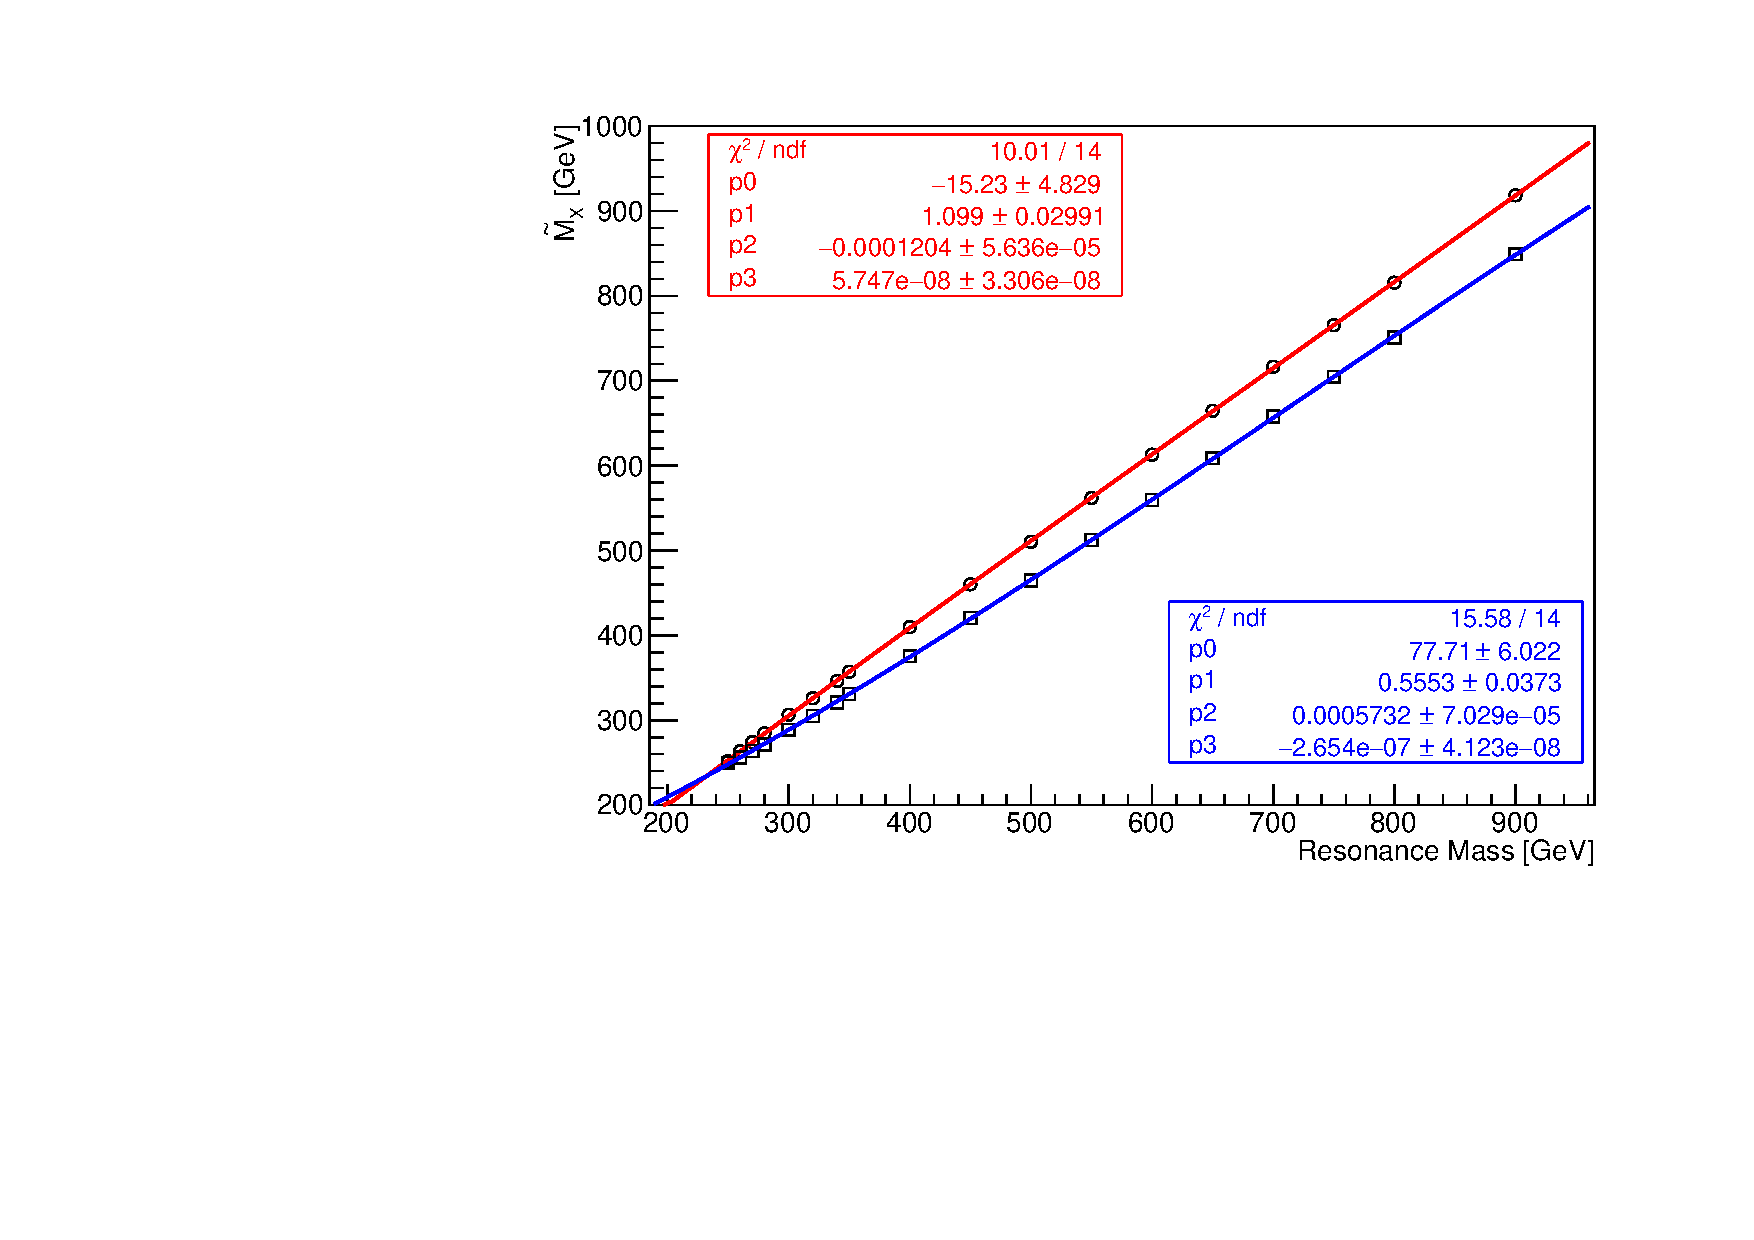
\includegraphics[width=0.45\textwidth]{figures/sec-window/fit_60_prime.pdf}\hfil

  \caption{Mass window sizes as a function of the resonance mass. }
  \label{fig:masswindowfit}
\end{figure*}

